\chapter{Evaluation}
\label{chapter:evaluation}

\guidance{%
  This is where Assessors will be looking for \textbf{signs of success} and for
  \textbf{evidence of thorough and systematic testing}. \textbf{Sample output},
  tables of timings and photographs of workstation screens, oscilloscope traces
  or circuit boards may be included.\\
  As with code, voluminous examples of sample output are usually best left to
  appendices or omitted altogether.\\
  There are some obvious questions which this chapter will address. \textbf{How
  many of the original goals were achieved? Were they proved to have been
  achieved? Did the program, hardware, or theory really work?}\\
  Assessors are well aware that large programs will very likely include some
  residual bugs. It should always be possible to demonstrate that a
  \textbf{program works in simple cases} and it is instructive to
  \textbf{demonstrate how close it is to working in a really ambitious case}.\\
}

\prechapter{%
  Here, the project's resounding success will be justified in relation to the
  aims of the project (as listed in~\ref{intro:aims}). Sample output will be
  shown and the interesting insights they provide will be explained. A
  comparison with existing tools will demonstrate the advantages of this project
  over existing tools (those mentioned in~\ref{prep:coqtools}).
}%

\section{Constructs Translated}

\subsection{Cognitive Walkthrough}

\subsection{Possible Extensions}

\section{Library of Queries}

\section{Sample output}\label{sec:sampleoutput}
\subsection{Small: CoqRegExp}

\subsection{Large: MathComp}

\section{A Comparative Analysis}\label{eval:compare}

\subsection{Features}

\begin{table}[tbp]
\centering
\caption{Comparison of Features}
\label{table:features}

\bigskip

\begin{tabular}{rccc}

  \toprule

  &
  \rot{Property 1} &
  \rot{Property 2} &
  \rot{Property 3} \\

  \midrule

  System 1        &       &       &  X    \\ 
  System 2        & X     & X     &  X    \\
  System 3        & X &   &  X            \\

  \bottomrule

\end{tabular}
\end{table}

\subsection{Performance}

\begin{figure}[tbp]
\centering

\caption{Comparison of Execution Times}
\label{fig:exectimes}
\bigskip

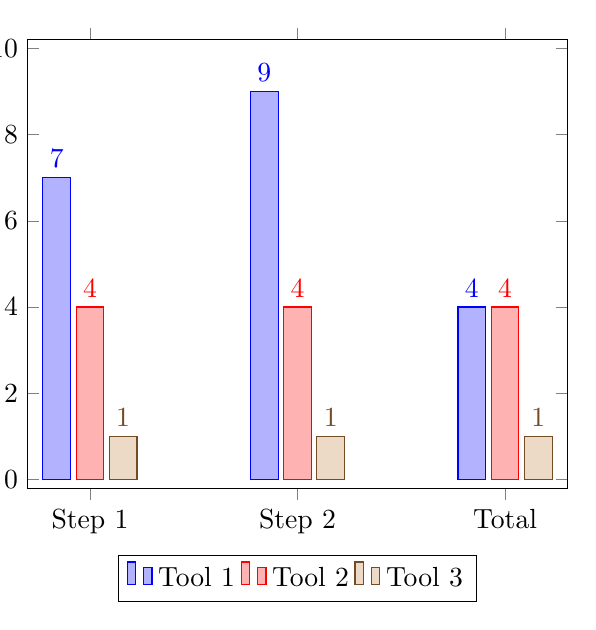
\begin{tikzpicture}[trim axis left]
	\begin{axis}[
		ybar,
		enlargelimits=0.15,
		legend style={at={(0.5,-0.15)},
		anchor=north,
		legend columns=-1},
		ylabel={time (ms)},
		symbolic x coords={Step 1,Step 2,Total},
		xtick=data,
		nodes near coords,
		nodes near coords align={vertical},
	]

	\addplot
		coordinates
			{(Step 1,7) (Step 2,9) (Total,4)};

	\addplot
		coordinates
			{(Step 1,4) (Step 2,4) (Total,4)};

	\addplot
		coordinates
			{(Step 1,1) (Step 2,1) (Total,1)};

	\legend
		{Tool 1,Tool 2,Tool 3}

	\end{axis}

\end{tikzpicture}
\end{figure}
